\documentclass{simple}

\title[Frame. Framing. Reframing]{Frame. Framing. Reframing}
\institute{Excursie PR708 \& friends}
\author[Răzvan Deaconescu]{Răzvan Deaconescu \\
razvan.deaconescu@cs.pub.ro}
\date{16 februarie 2019}

\begin{document}

\frame{\titlepage}

\begin{frame}{Întâmplări}
  \pause
  Megyn Kelly: ``You’ve called women you don’t like ‘fat pigs,’ ‘dogs,’ ‘slobs,’ and ‘disgusting animals’'' \\
  \pause
  Trump interrupted her with a quip: ``Only Rosie O’Donnell''. \\
  \vspace{0.5cm}
  \pause
  Hillary Clinton: (aprox.) ``How can someone who has been repeatedly accused of harassing women expect to become the President of the United States?'' \\
  \pause
  Donald Trump: ``Ask Bill.'' \\
  \vspace{0.5cm}
  \pause
  RD: ``Uite, așa a reușit Sergiu să se oprească să se masturbeze în PR708.'' \\
  \pause
  Sergiu: ``M-am oprit?''
\end{frame}

\begin{frame}{Frame is Everything}
  \pause perspectivă a interacțiunii (tranzacție socială) \\
  \pause contează mai mult în frame-ul cui se acționează decât cine are dreptate \\
  \pause cine se scuză se acuză \\
  \pause There is no such thing as bad publicity. \\
  \pause The only thing worse than being talked about is not being talked about.
\end{frame}

\begin{frame}{Frame Breaking}
  \pause
  supunere la presiune, cedarea punctului de vedere, persepectivei, frame-ului \\
  \pause
  enervare, pierderea controlului, submisie, scuze, ``opărire'', triggering
\end{frame}

\begin{frame}{Framing. Reframing}
  \pause
  framing: stabilirea perspectivei (tu inițiezi) \\
  \pause
  reframing: restabilirea perspectivei (tu reacționezi) \\
\end{frame}

\begin{frame}{Framing}
  Traian Băsescu: ``Ce blestem o fi pe acest popor de a ajuns să aleagă între doi foști comuniști, între Năstase și Băsescu?''
\end{frame}

\begin{frame}{Reframing: Tyrion Lannister}
  \pause
  Joffrey: ``I could tell the Hound to cut you in half!'' \\
  \pause
  Tyrion: ``That would make me a quarter-man. Just doesn't have the same ring to it.'' \\

  \vspace{1cm}

  \pause
  Tyrion Lannister: ``I am Tyrion, son of Tywin of Clan Lannister.'' \\
  \pause
  Shagga: ``How would you like to die, Tyrion, son of Tywin?'' \\
  \pause
  Tyrion Lannister: ``In my own bed, at the age of 80 with a belly full of wine and a girl's mouth around my cock.''
\end{frame}

\begin{frame}{Reframing: Scene din filme}
  \pause
  Crazy Stupid Love: https://www.youtube.com/watch?v=7kxOo5QotdA \\
  \pause
  Michael Corleone vs Hyman Roth: https://www.youtube.com/watch?v=pOoqlrhDabw \\
  \pause
  Tyrion vs Daenerys: https://www.youtube.com/watch?v=zikSq-QiA7U
\end{frame}

\begin{frame}{De ce framing/reframing?}
  \pause
  people test you, people push you \\
  \pause
  dominanță, putere, seducție \\
  \pause
  ``Everything in the world is about sex, except sex. Sex is about power.'' (Oscar Wilde) \\
  \pause
  respect \\
  \pause
  bonding
\end{frame}

\begin{frame}{You Will Be Tested}
  \pause
  test de congruență \\
  \pause
  vrei să vezi ce este cu adevărat cineva, care e adevărata fire \\
  \pause
  competiție pentru ierarhie \\
  \pause
  interacțiuni de toate felurile, cele mai evidente în interacțiuni intersexuale, politice și de dominanță/putere \\
  \pause
  joc social
\end{frame}

\begin{frame}{Testing}
  \pause
  JAIME: You clearly have no intention of saving your men’s lives. Why did you come treat with me? \\
  \pause
  BLACKFISH: Sieges are dull. And I wanted to see you in person, get the measure of you. \\
  \pause
  JAIME: Well, now you have. \\
  \pause
  BLACKFISH: Aye, now I have. I’m disappointed. \\

  \vspace{1cm}

  \pause
  (as Arthur has come to claim the Trident) Karathen: You do not belong here. I have guarded the Trident against false kings since the beginning and for a thousand years. I have seen the greatest champions try and failed, but never have I sensed one as unworthy as you. You dare to come here with your tainted mongrel blood to claim Atlantis’s greatest treasure? So be it. Half breed. \\
  \pause
  (as Arthur is trying to claim the Trident) Karathen: You thought yourself worthy? You thought yourself a king? You dishonour this place with your presence.
\end{frame}

\begin{frame}{Tehnici de reframing}
  \pause agree and amplify \\
  \pause disagree and amplify \\
  \pause non sequitur \\
  \pause assume the deal/sale \\
  \pause deflect \\
  \pause reflect \\
  \pause amused mastery \\
  \pause ambiguity \\
  \vspace{1cm}
  \pause
  contează contextul \\
  \vspace{1cm}
  \pause
  Crezi că rochia asta mă face grasă? \\
  \pause
  Ai fost mereu atât de prost? \\
\end{frame}

\begin{frame}{Bonding}
  \pause
  ball busting \\
  \pause
  ``Men bond by trading insults they don't really mean. Women do the same with compliments.''
\end{frame}

\begin{frame}{Mindset de framing}
  \pause
  relaxat \\
  \pause
  agresivitate controlată, rațională \\
  \pause
  autoritate \\
  \pause
  încredere / confidence \\
  \pause
  amuzant, bună dispoziție
\end{frame}

\begin{frame}{Mindset de reframing}
  \pause
  ZFG (\textit{Zero Fucks Given}) \\
  \pause
  outcome independence \\
  \pause
  abundance mentality \\
  \pause
  unfazed \\
  \pause
  confidence
\end{frame}

\begin{frame}{Anti-mindset de reframing}
  \pause pasiv agresivitate, defensivitate \\
  \pause sensibilitate, triggered \\
  \pause te ataci, agresivitate atacată \\
  \pause apologetic, scuze \\
  \pause reacții emoționale \\
  \pause frică puternică \\
  \pause lipsă de control \\
  \pause neediness, need to please, need to be praised \\
  \pause societal programming: be nice, be modest, be tolerant, don't attack others \\
  \pause self deprecation
\end{frame}

\begin{frame}{Cum faci bine framing/reframing?}
  \begin{itemize}
    \pause
    \item Înveți mai multe de la oameni care îți fac viața grea decât de la oameni care îți fac viața ușoară.
      \begin{itemize}
        \pause
        \item soră-mea, Alexandra Săndulescu, Răzvan Rughiniș, Costin Carabaș
        \pause
        \item intimidanți, se iau de tine, te testează des
      \end{itemize}
    \pause
    \item Simte-te bine în propria piele. Ești imperfect, ca noi toți. Acceptă asta. Îmbunătățește unde poți.
    \pause
    \item Listen to your gut. Fii congruent. Urmărește modele dar potrivește-le cu tine.
    \pause
    \item Observă. Învață.
    \pause
    \item Ai răbdare. Nu e ușor. Durează. Nu se termină niciodată.
  \end{itemize}
\end{frame}

\begin{frame}{Rețete}
  \begin{itemize}
    \pause
    \item Nu există rețete. You are never ready but you can be better.
    \pause
    \item dar \ldots
      \begin{itemize}
        \pause
        \item Progress breeds achievement. Achievement breeds confidence.
        \pause
        \item Urmăriți. Observați. Dezbateți. Învățați.
        \pause
        \item Interacționați cât mai mult. Discuții, activități, subiecte contondente, confruntaționale, controversate.
      \end{itemize}
    \pause
    \item Fiți asertivi. Spuneți ce vreți. Nu vă jenați. Nu există sacru. Spuneți pe bune.
    \pause
    \item Controlați și controlați-vă. Fiți stăpâni pe sine și pe situație.
    \pause
    \item Fiți amuzanți, bucurați-vă.
    \pause
    \item Nu e ușor.
  \end{itemize}
\end{frame}

\begin{frame}{Real Friends Test and Ball Bust}
  \begin{figure}
    \centering
    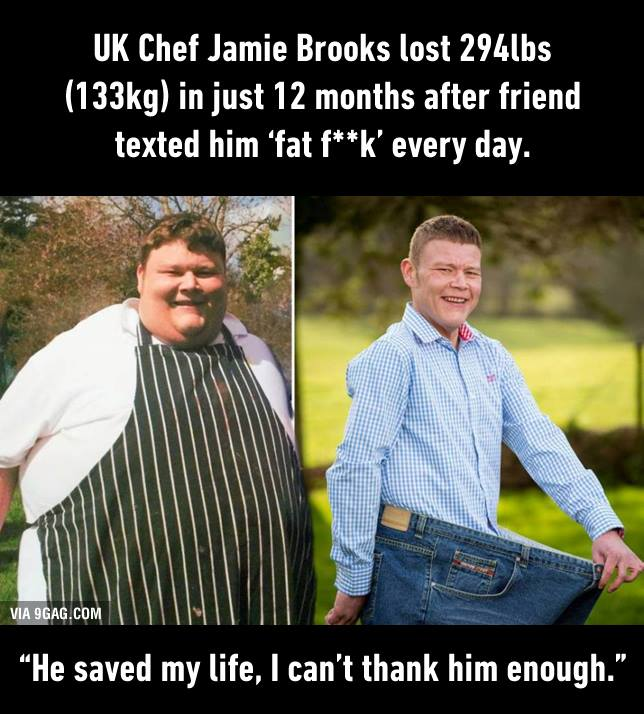
\includegraphics[width=0.4\textwidth]{img/getting-nasty-feedback.jpg}
  \end{figure}
\end{frame}

\begin{frame}{Real Friends Test and Ball Bust (2)}
  \begin{figure}
    \centering
    
\includegraphics[width=0.4\textwidth]{img/die-homo.png}
  \end{figure}
\end{frame}

\begin{frame}{}
  \pause
  \centering
  \LARGE{Frame. Reframe. Play the game.}
\end{frame}

\begin{frame}{Resurse și recomandări}
  \begin{itemize}
    \item slide-urile prezentării: \url{https://www.slideshare.net/razvandeaconescu/}
    \item Eric Berne: Games People Play
    \item Ed Latimore: Not Caring What Other People Think Is A Superpower
    \item Mark Manson: The Subtle Art of Not Giving a F*ck
    \item Robert Greene: The Art of Seduction
    \item Robert Cialdini: Influence: The Psychology of Persuasion
    \item Scott Adams (website, Twitter, videos)
  \end{itemize}
\end{frame}

\end{document}
